\documentclass[border=1pt]{standalone}
\usepackage{fontspec}
\usepackage[dvipsnames,svgnames]{xcolor} % Extended color support
\usepackage{tikz}
\usepackage{pgfplots}
\usepackage{amsmath}
\usepackage{amssymb}
\usepackage{mathtools}
\usepackage{unicode-math}
\usepackage{graphicx}
\usepackage{microtype}
\usepackage{enumitem}

\pgfplotsset{
  compat=1.18
}

%\setmainfont{Libertinus Sans}
%\setsansfont{Libertinus Sans}
%\setmonofont{Libertinus Mono}
%\setmathfont{Libertinus Math}

\setmainfont{Noto Sans}
\setsansfont{Noto Sans}
\setmonofont{Noto Sans Mono}
\setmathfont[
  Path=fonts/,
  Extension=.ttf
]{NotoSansMath-Regular}

\usetikzlibrary{
  calc,
  positioning,
  intersections,
  through,
  angles,
  quotes,
  arrows.meta,
  patterns,
  decorations.pathreplacing,
  decorations.markings,
  decorations.text,
  shapes,
  shapes.geometric,
  matrix,
  fit,
  backgrounds,
  fadings
}

\begin{document}
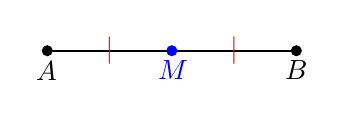
\begin{tikzpicture}[> =Latex]
  \tikzset{
    dimline/.style={
      arrows={Bar[length=0pt,width=20pt]}-{Bar[length=0pt,width=20pt]}
    },
    dot ends/.style={
      {Circle[length=2pt]}-{Circle[length=2pt]}
    },
  }
  \coordinate (a) at (0,0);
  \coordinate (b) at (90pt,0);

  \draw[thick] (a) node[below] {$A$} --(b) node[below] {$B$}
  node[midway,below,color=blue] {$M$}
  node[pos=0.25,color=red] {|}
  node[pos=0.75,color=red] {|};

  \fill[] (a) circle (2pt);
  \fill[] (b) circle (2pt);
  \fill[color=blue] ($(a)!0.5!(b)$) circle (2pt);
\end{tikzpicture}

\end{document}
